\documentclass[runningheads]{llncs}
\usepackage[T1]{fontenc}
\usepackage{graphicx}
\graphicspath{{./images/}}
% Used for displaying a sample figure. If possible, figure files should
% be included in EPS format.
%
% If you use the hyperref package, please uncomment the following two lines
% to display URLs in blue roman font according to Springer's eBook style:
%\usepackage{color}
%\renewcommand\UrlFont{\color{blue}\rmfamily}
%
\begin{document}
% Just after the begin
%\begin{document}
\begin{titlepage}
\centering
{\bfseries\LARGE International University of Ecuador \ 
Faculty of Technical Sciences  \par}
\vspace{1cm}
{\scshape\Large School of Mecatronics engineering \par}
\vspace{3cm}
{\scshape\Huge Industrial Automatization \par}
\vspace{3cm}
{\itshape\Large Group 4: Industrial Actuators \par}
\vfill
{\Large Author: \par}
{\Large Tomy Cuñas\par Pablo Guacho \par Sebastian Osorio \par}
\vfill
{\Large Sep 2022 - Jan 2023 \par}
\end{titlepage}
\newpage
%
\title{Industrial Actuators\thanks{UIDE.}}
%
\author{Sebastian Osorio\inst{1}\orcidID{0000-0003-0106-5482} }

\authorrunning{S. Osorio.}

\institute{International University of Ecuador, Quito Av. Jorge Fernández and Av. Simón Bolívar 170201, Ecuador
    \email{seosoriogu@uide.edu.ec}
    \url{https://www.uide.edu.ec/} }

\maketitle


\section{Introduction}
Industrial actuators are devices meant to do certain work, such as moving, controlling, or regulating. 
Are commonly used in industrial automation, robotics, and other applications.
It is controlled by a signal that is sent to the actuator. The signal can be electrical, hydraulic, pneumatic, or mechanical and
also it can be a combination of these signals\cite{RobotsYuk2017hydraulic}. Furthermore, the actuator can be controlled by a computer or by a human operator.
In a modern industrial automation actuators must have a feedback system to ensure that the actuator is working properly.

\section{Types of actuators}

\begin{enumerate}
    \item Motion\cite{RobotsYuk2017hydraulic,Near1996Piezoelectric}
    \begin{enumerate}
        \item \textbf{Linear:} They are actuators that move in a straight line. They are used to move objects in a straight line. 
        \item \textbf{Rotary:} They are actuators that rotate around an axis. They are used to move objects in a circular motion.
    \end{enumerate}
    \item Source of energy\cite{RobotsYuk2017hydraulic,Near1996Piezoelectric}
    \begin{enumerate}
        \item \textbf{Hydraulic: } They are actuators that use hydraulic energy to move. They are used in heavy machinery because they are very powerful. Even though they are very powerful, they are very slow.
        \item \textbf{Pneumatic:} They are actuators that use compressed air to move. They are fast and affordable used in small machinery. It is not very powerful. Even though it is not very powerful, it is very fast.
        \item \textbf{Electrical:} They are actuators that use electrical energy to move. Tend to be more precise and accurate than pneumatic actuators. Hover, they are more expensive.
        \begin{enumerate}
            \item \textbf{Electro-mechanical: } Are actuators that the control knob has been exchanged for an electric motor. They are used in small machinery. Resulting in the rotatory motion to be converted into a linear motion.
            \item \textbf{Electro-hydraulic: } Are actuators that use an electric motor to move a hydraulic piston. They are used in heavy machinery. Resulting in the rotatory motion to be converted into a linear motion but with more power.
        \end{enumerate}
        \item \textbf{Thermal and magnetic: }  usually consist of shape memory alloys that can be heated to produce movement. The motion of thermal or magnetic actuators often comes from the Joule effect. It can produce a wide range of motion while it is lightweight.
        \item \textbf{Mechanical Actuators: } Pure mechanical are actuators that use mechanical energy to move. Such as a lever, a crank, or a cam. They are used in small machinery. They are not very powerful and they are not very fast.
    \end{enumerate}
\end{enumerate}

\section{Most common actuators used in industrial automation}

As we mentioned before, there are many types of actuators. However, in this section we will talk about the most common actuators used in industrial automation.
Regarding linear motion actuators, the most common are the pneumatic Fig~\ref{fig:valve} and the hydraulic actuators. The pneumatic actuators are used in small machinery because
they are fast and affordable. The hydraulic actuators are used in heavy machinery because they are very powerful. Even though they are very powerful, they are very slow.
More over regarding rotary motion actuators, the most common are electric motors Fig~\ref{fig:stepMotor} hence they more precise and accurate than pneumatic actuators. Hover, they are more expensive.


\begin{figure}[!h]
    \centering
    \caption{Pneumatic linear actuator valve\cite{Valve}}\label{fig:valve}
    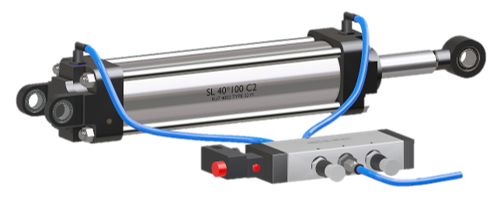
\includegraphics[scale = 0.6]{valve.png}
\end{figure}

\begin{figure}[!h]
    \centering
    \caption{Stepper motor\cite{Nema}}\label{fig:stepMotor}
    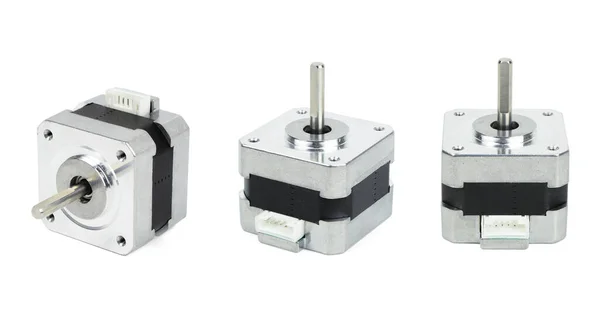
\includegraphics[scale = 0.55]{stepMotor.png}
\end{figure}


\section{Selection of actuators}

Depends on the application, the type of actuator to be used must be selected. The selection of the actuator is based on the following factors\cite{hines2017soft}:
\begin{enumerate}
    \item \textbf{Power:} The power of the actuator is the force that it can produce. The power of the actuator is measured in Newtons (N). The power of the actuator must be greater than the load that it will have to move.
    \item \textbf{Range of motion: } The range of motion of the actuator is the distance that the actuator can move. The range of motion of the actuator must be greater than the distance that the actuator will have to move.
    \item \textbf{Precision: } The quality, condition or fact of being exact and accurate to be controlled.
    \item \textbf{Environment: } Regarding the environment, the actuator must be selected according to the temperature, humidity, and dust of the environment. And even environmental concerns such as noise and vibration. 
    \item \textbf{Official guidelines: } The official guidelines are the standards that the actuator must meet. The most common are the ISO 9001, ISO 14001, NEMA and OHSAS 18001.
\end{enumerate}

\section{Example of actuator selection}

In this case considering a common application such as rotating an axis with a load of 10 N.
A stepper motor would be a good option because it is very precise and accurate. Considering only the load and a small power consumption the motor selected would be a stepper motor \textbf{SY42STH47-1206A} Fig~\ref{fig:StepMotorDiagram}. 
Looking at its data sheet 

\begin{figure}[!h]
    \centering
    \caption{Dimensions of the step motor 17HS4401}\label{fig:StepMotorDiagram}
    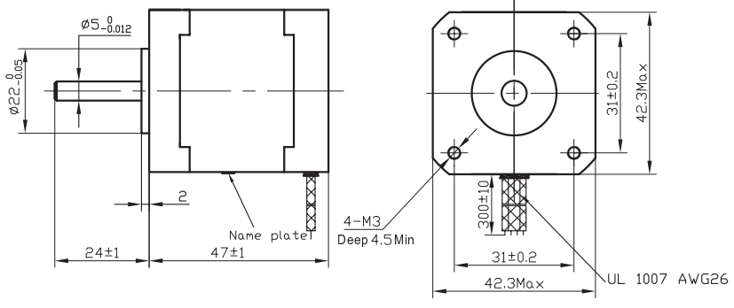
\includegraphics[scale = 0.7]{StepIsometric.png}
\end{figure}

Looking at the specs it has a radial force of 28 N and works at a voltage of 5 V at a current of 1.2 A. Resulting in the output torque graph Fig~\ref{fig:PullOutTorque}.

\begin{figure}[!h]
    \centering
    \caption{Dimensions of the step motor 17HS4401 }\label{fig:PullOutTorque}
    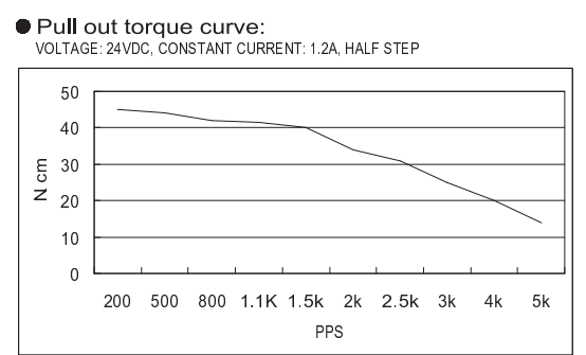
\includegraphics[scale = 0.7]{PullOutTorque.png}
\end{figure}




\bibliographystyle{splncs04}
 \bibliography{bibliography}
\end{document}